\section{Evaluation}
\subsection{Research Questions}
To evaluate our approach, we want to use our dataset of XWiki to answer the following \acp{rq}:
\begin{itemize}
    \item \ac{rq}1: \emph{How many bug tickets are found when selecting only a subset of tests using NLP-Clustering by Test Specification?}
    The goal of this paper is to discover whether a substantial amount of time and test executions can be saved when only selecting a portion of all tests when choosing the \ac{NLP}-based approach
    \item \ac{rq}2: \emph{How does the performance of NLP-based test selection compare with simpler, more naive methods of test selection in terms of bug detection?} We will compare how many more bug tickets we can cover with the new approach compared to naive approaches. This is done to show whether it is even worth it to implement something comparatively complex over something simple.
\end{itemize}

\subsection{Evaluation Metrics}
To evaluate how well our algorithm works, we want to find out how many bugs are
covered by a certain percentage of run tests. Our source also includes bug
tickets and we can link each test to its bug ticket. That way, we can go
through all \emph{n} selected tests, create a set of bug tickets covered, divide
its size by the number of all bug tickets and thereby know the percentage of bug
tickets covered. As we do not yet know how many tests should be selected, we
will go through all the percentage numbers from 10 to 70 in steps of ten and
see how many bug tickets have been covered by each number of tests and could then select the one appropriate for a given project.

\subsection{Comparison of Approaches}
To then find out how our algorithm compares to naive approaches we first have
to choose a naive approach. The first naive proposition that comes to mind is just
choosing \emph{n} random tests from our test cases. We will call this our "Completely Random" approach. Our second naive approach is only
possible with data that has some sort of categorization. As an example, the
test at
\begin{verbatim}
https://test.xwiki.org/xwiki/bin/view/File%20Manager%20Tests/Delete%20a%20file
\end{verbatim}
we mentioned earlier, is in the category \emph{P1.Extensions - File Manager
    Tests}. In total, there are 68 categories like this in our data set. As we can
assume similar bugs belong to similar test categories, this implementation
might lead to a well enough grouping of test cases.
In the end, we will compare selecting completely random tests from the entire dataset, selecting based on category and selecting based on the proposed NLP Approach.

\subsection{Results}

In the results, we chose to only select up to 70\% of tests, as clustering with KMeans did not provide enough separate clusters for 80\% or more of the test cases for our method, as our approach might lead to fewer distinct test-case vectors than actual test-cases. To avoid departing from the relatively simple and, as the results show, comparatively effective method, we decided to only select up to 70\% of tests. This limitation isn't problematic in our case, as the focus is to especially show the effectiveness of the approach for a more significant test case reduction than just 20\%.

We will now compare the mentioned methods based on their ability to discover bugs based on the appended bug tickets of the selected tests.
The first two methods in the table are our naive approaches explained in 4.3, while the latter one is the one explained in 3.2. In Table \ref{table:bug_ticket_coverage_comparison} and Figure \ref{fig:bugticketcoverage} we will call them as follows:
\begin{itemize}
    \item Completely Random, selecting test cases randomly from the entire dataset
    \item Category Random, selecting test cases randomly from each test category
    \item NLP Approach, being our presented approach with selecting tests by clustering test
          steps.
\end{itemize}

\begin{table}[H]
    \caption{Coverage of Bug Tickets by Percentage of Tests Run for Different Methods}

    \centering
    \renewcommand{\arraystretch}{1.5}  % Adjust the 1.5 to increase or decrease padding
    \begin{tabular}{|@{\hspace{5pt}}c@{\hspace{5pt}}|@{\hspace{5pt}}c@{\hspace{5pt}}|@{\hspace{5pt}}c@{\hspace{5pt}}|@{\hspace{5pt}}c@{\hspace{5pt}}|}  \hline
        Percentage of Tests Run & Completely Random & Category Random & NLP Approach \\ \hline
        10\%                    & 14.22\%  & 15.14\%  & 18.81\%  \\ \hline
        20\%                    & 26.15\%  & 27.75\%  & 36.24\%  \\ \hline
        30\%                    & 37.84\%  & 38.53\%  & 51.61\%  \\ \hline
        40\%                    & 47.25\%  & 47.94\%  & 59.86\%  \\ \hline
        50\%                    & 52.98\%  & 54.82\%  & 72.48\%  \\ \hline
        60\%                    & 69.95\%  & 68.35\%  & 80.96\%  \\ \hline
        70\%                    & 73.62\%  & 70.87\%  & 83.03\%  \\ \hline
    \end{tabular}
    \label{table:bug_ticket_coverage_comparison}
\end{table}

\begin{figure}[H]
    \centering
    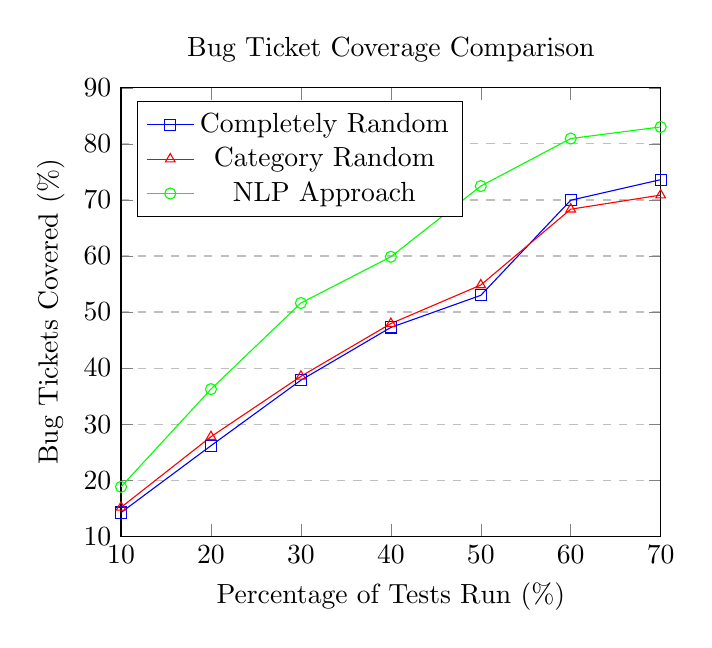
\begin{tikzpicture}
        \begin{axis}[
                title={Bug Ticket Coverage Comparison},
                xlabel={Percentage of Tests Run (\%)},
                ylabel={Bug Tickets Covered (\%)},
                xmin=10, xmax=70,
                ymin=10, ymax=90,
                xtick={10,20,30,40,50,60,70},
                ytick={10,20,30,40,50,60,70,80,90},
                legend pos=north west,
                ymajorgrids=true,
                grid style=dashed,
            ]

            \addplot[
                color=blue,
                mark=square,
            ]
            coordinates {
                    (10,14.22)(20,26.15)(30,37.84)(40,47.25)(50,52.98)(60,69.95)(70,73.62)
                };
            \addlegendentry{Completely Random}

            \addplot[
                color=red,
                mark=triangle,
            ]
            coordinates {
                    (10,15.14)(20,27.75)(30,38.53)(40,47.94)(50,54.82)(60,68.35)(70,70.87)
                };
            \addlegendentry{Category Random}

            \addplot[
                color=green,
                mark=o,
            ]
            coordinates {
                    (10,18.81)(20,36.24)(30,51.61)(40,59.86)(50,72.48)(60,80.96)(70,83.03)
                };
            \addlegendentry{NLP Approach}

        \end{axis}
    \end{tikzpicture}
    \caption{Comparison of different test selection approaches in terms of bug tickets covered.}
    \label{fig:bugticketcoverage}
\end{figure}

Table \ref{fig:bugticketcoverage} shows that a \ac{NLP}-based selection of 30\% of the tests achieves a bug detection quota of 51.61\%, while 50\% results in a quota of 72.48\%.
This means we can still detect nearly $\frac{3}{4}$ of all bugs when only executing $\frac{1}{2}$ of all tests.
We can also see that the naive approaches are very similar to each other and perform worse than the \ac{NLP}-based selection. 
For the first naive approach, Table \ref{fig:bugticketcoverage} shows that a random selection of 30\% of tests results in a bug detection quota of 37.84\%, while a selection of 30\% of tests results in 52.98\% of bug tickets covered.

The next naive approach was to select based on categories. Selecting 30\% of test cases from separate categories showed a bug detection quota of 38.53\%, while a selection of 50\% covered 54.82\% of bug tickets.